\section{Durchführung}

\subsection{Aufbau}
Der Versuch besteht aus einer Kupfer-Röntgenröhre, einem Geiger-Müller-Zählrohr und einem LiF-Kristall,
die in einem Röntgengerät integriert sind, vgl. Abbildung \ref{fig:der_geraet}.
Das Röntgengerät wird dabei über einen Computer mit Hilfe des Programmes \texttt{measure} bedient.
Dort wird unter \enquote{Messgeräte} das Röntgengerät ausgewählt.
Anschließend kann die Messart, der Drehmodus, der Kristallwinkel und die Integrationszeit gewählt werden.
Die Messart sollte dabei auf \enquote{Spektren} stehen.

\noindent
Die Beschleunigungsspannung wird für alle Messungen auf \qty[]{35}{\kilo\volt} und der Emissionsstrom auf \qty[]{1}{\milli\ampere} eingestellt.
Vor den Messungen wird überprüft, ob die \qty[]{1}{\milli\meter} Blende und der LiF-Kristall in der Halterung stecken.
Ferner wird kontrolliert, ob die Schlitzblende senkrecht zur Drehrichtung sitzt.

\noindent
Zur Messung der Absorption können diverse Blenden mit verschiedenen Absorptionsmaterialen vor das Zählrohr geschraubt werden.

\begin{figure}[H]
    \centering
    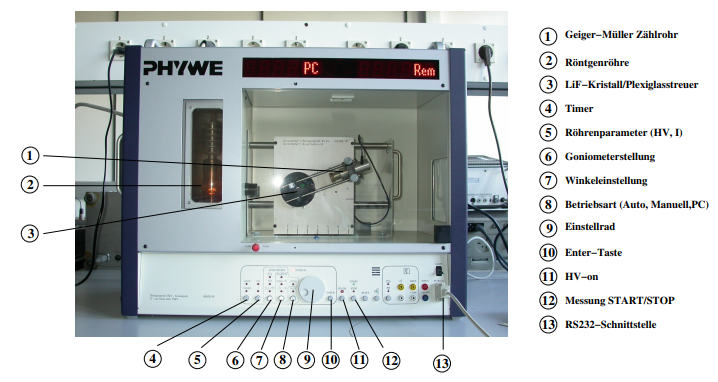
\includegraphics[height = 6.5 cm]{Abbildungen/der_geraet.png}
    \caption{Das Röntgengerät mitsamt seiner Bestandteile \cite{man:v602}.}
    \label{fig:der_geraet}
\end{figure}


\subsection{Überprüfung der Bragg-Bedingung}
Zur Überprüfung der Bragg-Bedingung wird der Kristall auf einen \enquote{festen Kristallwinkel} von \qty[]{14}{\degree} eingestellt.
Bei einer Integrationszeit von \qty[]{5}{\second} wird in einem Winkelbereich von \qtyrange[]{26}{30}{\degree} mit einem Winkelzuwachs
von \qty[]{0.1}{\degree} die Strahlungsintensität der Röntgenstrahlung gemessen. 


\subsection{Emissionsspektrum der Kupfer Röntgenröhre}
Zur Messung des Emissionsspektrums der Kupferröhre wird im Programm der \enquote{2:1 Koppelmodus} ausgewählt.
Dabei wird die erste Beugungsordnung im Winkelbereich \qtyrange[]{4}{26}{\degree} in \qty[]{0.2}{\degree} Schritten gemessen.
Die Integrationszeit wird dazu auf \qty[]{5}{\second} eingestellt.

\noindent
Im nächsten Schritt werden anhand der vorherigen Messung die ungefähre Lage der $K_\alpha$- und $K_\beta$-Linien abgelesen
und in ihrem Bereich ein Detailspektrum aufgenommen, damit die beiden Linien genauer bestimmt werden können.
Hierzu wird die Schrittweite auf \qty[]{0.1}{\degree} angepasst.


\subsection{Absorptionsspektren verschiedener Materialien}
Für insgesamt vier Materialien (Zink, Brom, Strontium, Zirconium) werden die Absorptionsspektren gemessen.
Dafür werden die jeweiligen Absorber vor das Zählrohr gesetzt und in \qty[]{0.1}{\degree} Schritten bei einer Integrationszeit 
von \qty[]{20}{\second} die jeweiligen Intensitäten gemessen.
Anhand von Tabelle \ref{tab:vorbereitung} werden hierfür geeignete Winkelbereiche gewählt.